\documentclass[border=0mm,tikz]{standalone}
\usepackage{csquotes}
\usepackage[backend=biber,style=numeric,sorting=none]{biblatex}

\usepackage{siunitx}
\usepackage{tikz}
\usetikzlibrary{decorations.pathmorphing,patterns}
\usetikzlibrary{shapes.geometric, arrows.meta}
\usetikzlibrary{positioning}

\usepackage{amsmath}
\usepackage{upgreek}
\usepackage{svg}

\usetikzlibrary{3d}
\usetikzlibrary{calc}

\tikzset{
box/.style={
	rectangle,
	rounded corners=4pt,
	minimum width=3cm,
	minimum height=1cm,
	text centered,
	draw=black!70,
	line width=0.95pt,
	fill=gray!5,
	inner sep=4pt
},
circlebox/.style={
	circle,
	minimum size=1.5cm,
	text centered,
	draw=black!70,
	line width=0.95pt,
	fill=gray!5,
	inner sep=1pt
},
arrow/.style={
	thick,
	->,
	>=Stealth,
	draw=black!70,
	line width=1pt,
	line cap=round,
	line join=round,
	shorten <=1pt,
	shorten >=1pt
}
}

\begin{document}

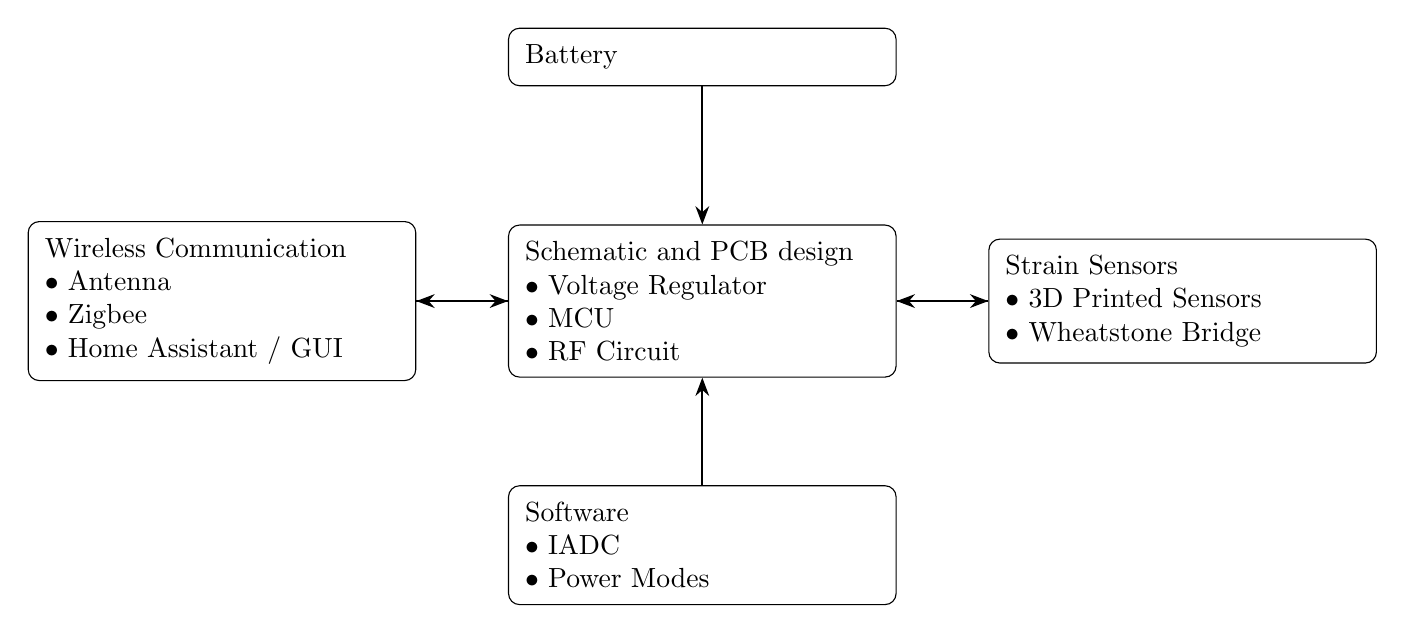
\begin{tikzpicture}[
  node distance=3.1cm,
  box/.style={
    draw,
    rounded corners,
    rectangle,
    text width=4.5cm,
    align=left,
    inner sep=6pt
  },
  arrow/.style={-Stealth, thick}
]

\node (Battery) [box] {Battery};
\node (PCB) [box, below of=Battery] {Schematic and PCB design\\
  \(\bullet\) Voltage Regulator\\
  \(\bullet\) MCU\\
  \(\bullet\) RF Circuit
  };
\node (Wireless) [box, left of=PCB, xshift=-3cm] {Wireless Communication\\
  \(\bullet\) Antenna\\
  \(\bullet\) Zigbee\\
  \(\bullet\) Home Assistant / GUI
};
\node (Software) [box, below of=PCB] {Software\\
  \(\bullet\) IADC\\
  \(\bullet\) Power Modes
};
\node (Sensor) [box, right of=PCB, xshift=3cm] {Strain Sensors\\
  \(\bullet\) 3D Printed Sensors\\
  \(\bullet\) Wheatstone Bridge
};

% All nodes -> PCB
\draw[arrow] (Battery.south)  -- (PCB.north);
\draw[arrow] (Software.north) -- (PCB.south);

% Bidirectional links (offset so both arrows are visible)
\draw[arrow] (Wireless.east) to[out=0, in=180] (PCB.west);
\draw[arrow] (PCB.west)      to[out=180, in=0] (Wireless.east);

\draw[arrow] (Sensor.west) to[out=180, in=0] (PCB.east);
\draw[arrow] (PCB.east)    to[out=0, in=180] (Sensor.west);

\end{tikzpicture}

\end{document}